\documentclass{llncs}

\usepackage{times}
\usepackage{graphicx}
\usepackage{url}
\usepackage{verbatim}
\usepackage{fullpage}

\title{PseudoID: Enhancing Privacy for Federated Login}
\author{Arkajit Dey\inst{1} and Stephen Weis\inst{2}}
\institute{Massachusetts Institute of Technology, Cambridge, MA, USA 02139
\and
Google Inc., Mountain View, CA, USA 94043}

\begin{document}

\maketitle

\begin{abstract}
  This paper proposes a privacy-preserving federated login system
  named \emph{PseudoID}. PseudoID protects both individual user
  privacy and identity providers data. This system is based on blind
  digital signatures and is compatible with a popular federated login
  system named OpenID. We propose several extensions and discuss some
  of the practical challenges that must be overcome to further protect
  user privacy.
\end{abstract}

\section{Introduction}
\label{sec:intro}

Internet users often manage login credentials for many accounts across
multiple web sites. This is both an inconvenience and a potential
security risk, as users often resort to reusing passwords. Users also
become accustomed to typing usernames and passwords in many different
interfaces, making them more susceptible to phishing, that is, having
their credentials stolen by spoofed websites.

This has led to several efforts to create web single sign-on (SSO)
systems. One SSO model is for users to have a single \emph{identity
  provider} (IDP) for all logins. Arbitrary web sites may then become
\emph{relying parties} (RPs), who delegate logins to the IDP. The IDP
handles authenticating the user and attesting an identity back to the
RP.

Some proposals, such as Windows Live ID \cite{MSPass} or Facebook
Connect \cite{FBConnect}, relied on a centralized IDP. Other systems,
such as OpenID \cite{OID}, allow users to have identities from among a
federation of IDPs. Federated login systems like OpenID offer more
flexibility to end users, since they are able to choose among many
identity providers. Large webmail providers like Yahoo, Google, and
MSN have all adopted OpenID \cite{YOP,Sac08,WLOP08} and are capable of
serving as identity providers for hundreds of millions of users.

While federated login systems like OpenID may streamline logins, they
may create risks to user privacy. The core problem in both centralized
and federated login systems is that all of a user's logins to relying
web sites must flow through an identity provider. A user's IDP can
easily link together the various websites that the user visits. An
IDP could, for example, release data about which sites users visited
without user consent.

In a federated system, users could avoid identity providers
that abused privacy and choose to use reputable firms. Unfortunately,
honest identity providers may still be compromised and leak logs, or
otherwise be compelled to reveal logs.

Besides simply revealing which sites a user visits, IDPs often reveal
personal information about users through extensions like OpenID
attribute exchange (AX) \cite{AX} or simple registration (SREG)
\cite{Sreg}. The goal of this exchange is typically to pass
information like an email address, real name, or birthdate from an
identity provider to a web site. Automatically obtaining these data
can greatly streamline the user sign-up process for relying parties.

Although most IDPs will prompt users whether they want to reveal this
information, they could reveal whichever data they want to a relying
party. Thus, there is no way for a user to \emph{selectively disclose}
certain properties (e.g. age, gender, etc.) about themselves to an
RP. Much work has gone into developing cryptographic schemes for
selective disclosure \cite{CaLy01,CaLy04,CHL05,CaGr08}, but these have
yet to be widely adopted in practice.

In this paper, we outline a privacy-preserving federated login system
called PseudoID and offer a sample implementation as a pseudonymous
OpenID provider. The system utilizes blind signatures \cite{Cha82} as
part of a blind signature service. This service allows users to
generate a pseudonym that can be used to login to relying parties, but
cannot be linked to their true identity. We also propose 
extensions based on zero-knowledge proofs \cite{GMR89} to support
selective disclosure of user properties.

\section{Federated Login Overview}
\label{sec:fedlogin}

Web users who want to use a particular website most often authenticate
themselves directly to the site by entering a username and
password as in Figure \ref{fig:passwd}. Maintaining many sets of user
credentials across different sites carries a burden for the user, and can
lead to password reuse.

Websites must carry the burden of creating accounts, storing
credentials, and authenticating users. Account creation, or
``on-boarding'', is often a large barrier to signing up new users. It
is not uncommon for the over half of sign-up attempts to be
abandoned. 

\begin{figure}
  \centering
  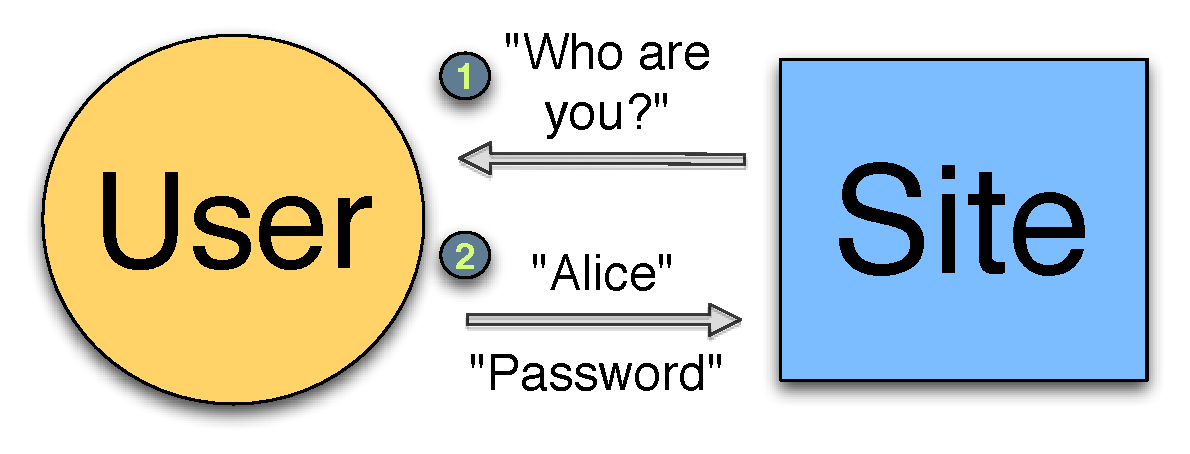
\includegraphics[scale=0.5]{figs/fig-passwd-color.pdf}
  \caption{A typical  web login system where users log into websites
    by entering site-specific credentials.}
  \label{fig:passwd}
\end{figure}

Federated login systems, on the other hand, extract authentication as
a service in its own right. Just as websites rely on third-party services
for traffic analysis, CAPTCHA verification, or file hosting, they can
also rely on separate services for authentication.

Federated login adds a third party to the interaction between the user
and the website: the \emph{identity provider} (IDP). Instead of
authenticating herself to the website directly, the user authenticates
herself to the IDP. The IDP then returns a user identifier to the
website. Thus, the website is often referred to as the \emph{relying
  party} (RP) since it relies on the identity provider for
authentication.

\begin{figure}
  \centering
  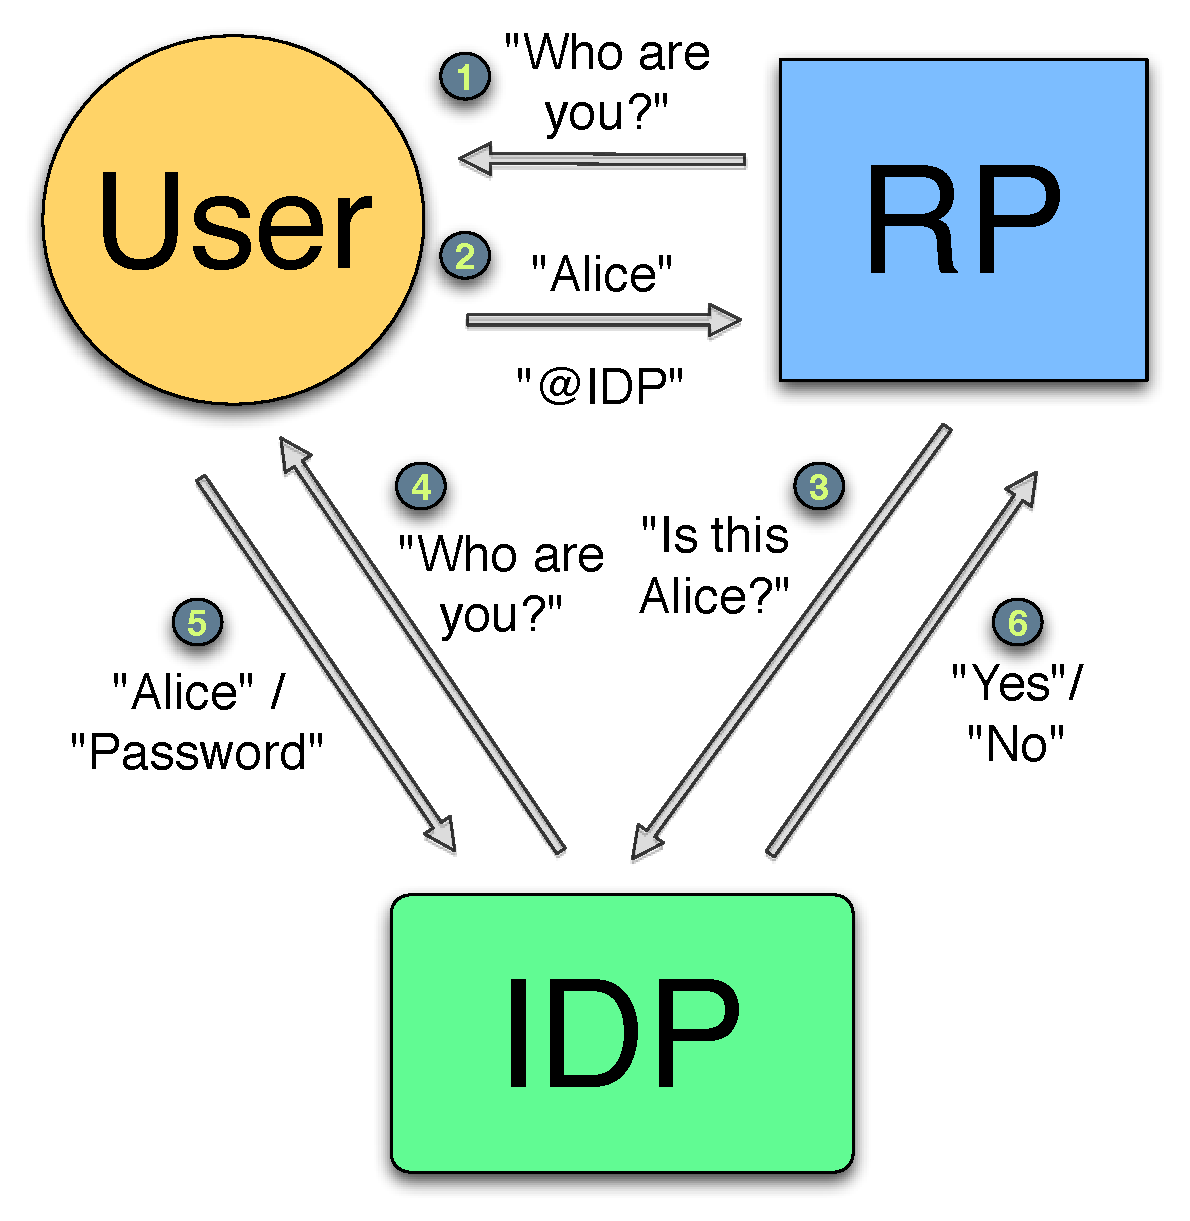
\includegraphics[scale=0.5]{figs/fig-fedlog-color.pdf}
  \caption{A federated login system: the relying party (RP) redirects
  the user to her identity provider (IDP) for authentication.}
  \label{fig:fedlog}
\end{figure}

Federated login alleviates the need for websites to store user
credentials, making them less desirable targets for hackers who want
to hijack user accounts. The user benefits from federated login too.
Instead of managing separate login credentials for every website he
wants to use, the user can just log into a single IDP.

Systems like Facebook Connect and OpenID 2.0 are able to offer
one-click logins for relying parties, which greatly simplifies the
login process. For example, Plaxo, a social networking and address
book site, performed a two-click OpenID login experiment where 92\% of
users successfully completed registration after starting the signup
process \cite{Ki09}. In contrast, on-boarding abandonment rates of
50\% are common for many websites.

Accordingly, federated login systems are being adopted by a growing
number of internet sites, particularly by large webmail providers and
social networks.  Several different federated login technologies have
arisen over the years, such as Microsoft Passport (now Windows Live
ID), OpenID, Facebook Connect, and SAML.

However, popular federated login systems have generally been designed
without privacy as a primary concern. Subsequently, current
widely-used federated login systems which could put sensitive user
data at risk. The problem of user privacy is indeed magnified in
federated login systems since identity providers act as stewards of
user data for multiple websites. This not only makes IDPs more
appealing targets to attackers, but also more likely to be subpoenaed
for user records.

\subsection{OpenID: A web-based federated login system}

OpenID is a popular federated login system that we focus on for a
proof of concept implementaion \cite{OID}. In OpenID, users can claim
identifiers in the form of URIs. To login to a website that supports
OpenID, the user enters his OpenID URI and the RP redirects him to
his identity provider's page. The IDP authenticates the user through
its choice of authentication system (e.g. passwords, smart cards,
etc.) and then returns the user to the RP with either a positive or
negative assertion that the user owns the claimed identifier. If the
RP receives a positive assertion from the IDP, it may allow the user
to enter the site under the name of the claimed identifier.

With the advent of OpenID 2.0 \cite{OID2}, the protocol also began to
support the concept of \emph{directed identity} \cite{Cam06} or
\emph{private digital addresses} through a new feature called
\emph{identifier select} \cite{RR06}.  This allows the user to just
specify the URI of his identity provider instead of claiming a
personal identifier when logging into a website. The site then
redirects the user to the IDP as before, but the IDP now has the
opportunity to select an identifier for the user. Upon successfully
authenticating the user, the IDP returns the selected identifier to
the site.

This allows the IDP more flexibility in selecting identifiers for its
users. For example, the IDP may decide to return a different
identifier for the same user for different RPs in order to implement
true directed identity as defined in Kim Cameron's Laws of Identity
\cite{Cam06}. Indeed, some OpenID providers like Google do return a
per site unique identifier rather than a globally unique identifier
for its users.

\subsection{Privacy Concerns in Federated Login}

In federated login systems, users entrust identity providers to manage
their identity, so privacy concerns may seem relatively minor. After
all, in OpenID and most other major single sign-on systems, a
malicious identity provider could easily impersonate users to relying
parties. However, even if an identity provider is not corrupt, there
are privacy concerns for \emph{honest, but retentive} providers who
may reveal user data due to a security breach or a legal
subpoena.

The core privacy issue with widely-deployed federated login systems
is that a user's identity can be correlated with the sites he logs
into. For example, OpenID identity providers will authenticate users,
then redirect them directly back to a relying party. This makes it
trivial to know all the web sites a user logs into. The same
is true for Live ID or Facebook Connect.

One might develop a different federated login flow where a user acted
as an intermediary between relying parties and identity providers. The
user could avoid passing any information about the specific relying
party to the identity provider. In this case, the identity provider
might return an anonymized identifier via the user to the relying
party. However, if the provider colluded with the relying party, they
could link the user's real identity with the account on the RP.

Alternatively, an identity provider could abstain from logging, could
try to anonymize or delete identifying information, or could simply
destroy logs completely. Logs are retained for many valid reasons
including analytics, diagnostics, and security auditing. In practice,
abstaining from logging is generally not a viable option.

Removing or anonymizing identifying information ex post facto is one
option, but has proved difficult in practice. Supposedly anonymized
logs released by AOL \cite{BarZel06} and Netflix \cite{NaSh08} were
both de-anonymized to some extent. An identity provider would need to
be vigilant and thoroughly scrub logs. They would also need to ensure
that identifying data was not being unintentionally logged by an
unrelated service or a different layer of the stack.

Another issue is that both logs anonymization and destruction may be
subject to data retention laws that specify minimum retention periods
\cite{EUDir}. IDPs may be legally compelled to collect identifying
data and retain it for a minimum period. In some jurisdictions,
authorities have broad powers to rapidly sieze these data, often
without user knowledge.

Given these considerations, we will focus on privacy in a setting where:
(1) identity providers are unable to assure that logs are not retained, and
(2) identity providers may be compelled to reveal logs at some time.

There are several real-world risks where \emph{honest, but retentive}
identity providers may threaten user privacy. One risk is simply if
the provider were compromised and logs were leaked by an
attacker. Another risk is for providers operating in jurisdictions
where logs may be seized without due legal process. 

Identity providers may have an interest in \emph{not} being able to
link a particular user's identity to logins on a relying party. An
identity provider may want to provably show that they cannot link
logins on a relying party to a particular user. With this in mind, we
informally define what it means for an idenity provider to be
\emph{private} in Section \ref{sec:private-fed-login}. Section
\ref{sec:pseudoid} propose a practical system that meets this
definition.

\section{Properties of Private Federated Login}
\label{sec:private-fed-login}

For the scope of this paper, we are going to focus on privacy in
federated login systems with an OpenID-like login flow illustrated in
Figure \ref{fig:fedlog}. The relevancy to other types of federated
login systems may vary. 

We assume that identity providers have a set of users that can be
thought of as ``real'' identities. Users may possess credentials which
are presented to identity providers for authentication. If the credentials
are valid, identity providers will return some identifier to a relying
party. This identifier may be of any form, i.e. a ``real'' username, a
pseudonym, a value derived from the credentials, or even a random
value. In order to contrast these different behaviors, we will first
state several informal properties.

\begin{definition}[One-wayness]
\label{def:ownership}
An identity provider is one-way if given a specific identifier,
attackers have no significant ability to cause identity providers to
return that value.
\end{definition}

One-wayness means that users actually ``own'' their identities and
people cannot imitate them on relying parties, e.g. as with a familiar
username/password login. A trivial example of an identity provider
that is \textit{not} one-way is one where an IDP will assert any
identity without authorizing the user.  We'll refer to this as the
``Yes IDP''. Users of a Yes IDP could log into RPs with arbitrary
identities, but would not be able to prevent other people from using
the same identities.

\begin{definition}[Consistency]
\label{def:consistency}
An identity provider is consistent if users may present credentials
that will return the same identifier over multiple sessions.
\end{definition}

The consistency property means that users can have long-lived
identities on relying parties. That is, users can log in as the same
identity to a relying party any number of times. A trivial
inconsistent IDP would be one which returned a random value for each
login, or a ``Random IDP''. Users of a Random IDP would be anonymous
on relying parties and could not be linked to their real identities,
but would not be able to establish long-lived accounts on RPs.

\begin{definition}[Unlinkability]
\label{def:unlinkability}
An identity provider is unlinkable if given a transcript of an
authentication event and a set of users, an attacker has no
significant advantage in distinguishing the user being authenticated.
\end{definition}

Unlinkability is intended to capture the notion that an attacker who
obtains access logs from an identity provider and relying party should
not be able to tell which ``real'' user was logging in.

OpenID identity providers are generally linkable in practice, although
there are exceptions. An attacker obtaining a user's credentials or
IDP access logs would be able to trivially see which user was
associated with a particular identity on a relying party.

Note that this property is not specific to OpenID or a flaw in the
OpenID protocol. Instead, it's an artifact of how real world identity
providers typically authenticate users: with usernames and
passwords. For example, an attacker may observe ``Alice'' authenticate
herself to an IDP and the identity ``Bob'' returned to a relying
party; linking her real identity to her pseudonym.

Thus, an unlinkable relying party must not require any identifying
information about their real users during the federated login
protocol. The Yes and Random IDPs mentioned before are in fact
unlinkable, but are not practical in many use cases since they are
respectively not one-way or consistent. A practical unlinkable system
must be both one-way and consistent. We will present such a system in
Section \ref{sec:pseudoid}.

\section{PseudoID: A privacy-preserving federated login system}
\label{sec:pseudoid}

PseudoID is designed to be a one-way, consistent, and unlinkable
federated login system. It consists of a token service used during
setup, and a private identity provider used for sign-ons. The user has
an account with the token service, which may be a persistent, ``real''
identity like an email address. During setup, the user logs on to the
token service using a familiar authentication scheme, such as entering
a username and password.

The user then requests an access token from the token service that is
bound to a desired pseudonym. When logging into a relying party, the
user presents this token to an identity provider. The identity
provider will verify the authenticity of the token and return the
user's pseudonym to the relying party.

To be unlinkable, the access tokens must be generated such that even
if both the token service and identity provider are compromised, the
user's ``real'' identity with the token service cannot be linked to
their pseudonyms on different relying parties. PseudoID achieves this
property by employing \textit{blind signatures}.

\subsection{Blind Signatures}
\label{section:blind-sigs}

Traditional public key digital signature schemes \cite{DH76} consist
of a private signing function $\sigma$ known only to the signer and a
public verifying predicate $V$. Then for any message $m$ that is
provided to the signer to be signed, a verifier can check that $V(m,
\sigma(m))$ is true.

Blind signature systems \cite{Cha82} augment this traditional scheme
with a blinding function $B$ and its inverse unblinding function
$B^{-1}$, such that $B^{-1}(\sigma(B(m)) = \sigma(m)$ and both
functions are known only to a user getting a message signed.

The user wishes to obtain a signature $\sigma(m)$ on some message
$m$ without revealing the contents of $m$ to the signer. Thus, the
user sends the blinded message, $B(m)$, to the signer. The blinded
message leaks no information about $m$ to the signer. The signer then
signs the blinded message and returns $\sigma(B(m))$ to the
user. Finally, the user unblinds this signed message to
obtain $$B^{-1}(\sigma(B(m))) = \sigma(m),$$ a valid signature on $m$
that can be publicly verified.

One example of a blind signature system is Chaum's RSA blind signatures. In a
standard RSA digital signature system, the public parameters are a modulus $n$
and an exponent $e$. Only the signer knows the private exponent $d$.

To blind a message $m$ prior to sending it to the signer, the user
multiplies it by a random blinding factor $r$ to produce $B(m) =
mr^e$. The signer signs $B(m)$ to produce $$m^d r^{ed} \equiv m^d r
\pmod n$$ by Euler's theorem. Since the user can compute $r^{-1}$,
he can unblind the returned signature to obtain $$m^d \pmod n,$$ a
valid signature on the original message $m$.

%TODO(arkajit): cite more blind sig scheme examples like El Gamal?
%Maybe not worth the time.

\subsection{Blind Token Service}

PseudoID employs a blind signature service (BSS) or \emph{blind
  signer} that generates blinded access tokens. These tokens are
redeemed with an identity provider and used to derive identifiers that
are returned to relying parties. This setup phase is outlined in
Figure \ref{fig:bss-setup}.

During a setup phase, the user will visit the blind signer and login
to an existing account. The user then selects a pseudonym that they
want to use on a relying party. This pseudonym is bundled into an
access token that the blind signer will sign.

To prevent the signer from being able to link a user with her
pseudonym, the user first blinds the token before sending it to the
blind signer. The blind signer will sign this token without knowing
its contents and return it to the user. Upon receiving the singed
token back from the service, the user unblinds it to obtain a signed
token that contains the user's chosen pseudonym. Note that the blind
signer will not see the user's pseudonym in the clear; it will only
see the blinded token.

\begin{figure}
  \centering
  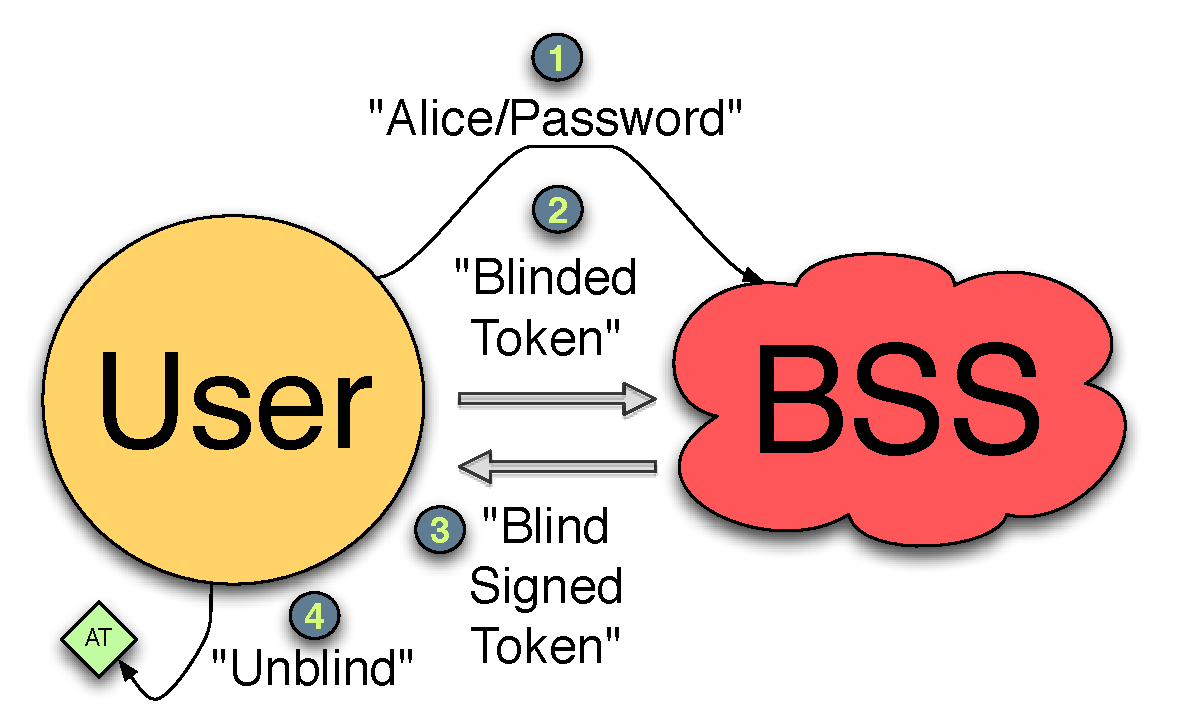
\includegraphics[scale=0.6]{figs/fig-bss-setup-color.pdf}
  \caption{Blind Signer Setup: (1) User first authenticates herself to the BSS
  normally. (2) Then the user sends the BSS a blind token to sign. (3) The BSS
  signs the token and returns it. (4) The user unblinds the blind signed token
  to obtain a valid, untraceable access token (AT).}
  \label{fig:bss-setup}
\end{figure}

\subsection{Private Identity Provider}

The identity provider relies on the blindly signed tokens to be able
to authenticate users without forcing them to reveal their
identity. When a user is redirected to her identity provider by a
relying party, the provider checks whether the user has an access
token that has been signed by the blind signer.

The signature on the token may be either publicly verifiable or
privately verifiable. In the former case, the identity provider can
verify the signature on the access token using the blind signer's
public key. In the latter case, the identity provider could send the
token to the blind signer and ask them whether they signed it. The
sign-on process using an access token in the publicly verifiable case
is illustrated in Figure \ref{fig:bss-signon}.

\begin{figure}
  \centering
  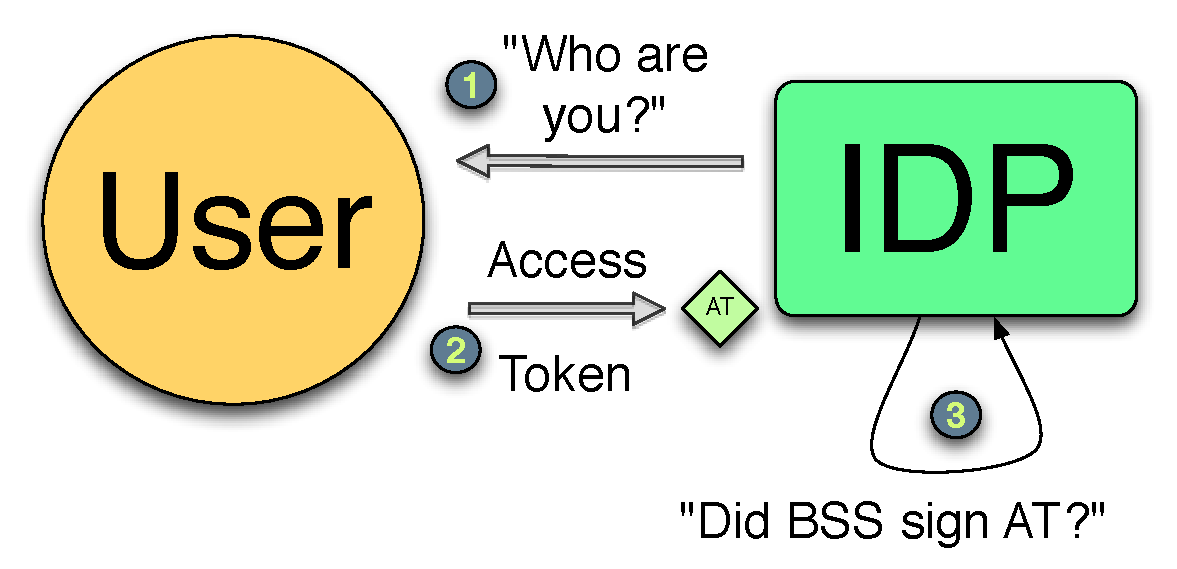
\includegraphics[scale=0.6]{figs/fig-bss-signon-color.pdf}
  \caption{Identity Provider Signon with Blind Signed Access Token: (1) IDP asks
  users to authenticate (2) User supplies access token rather than true identity
  or credentials (3) IDP verifies whether BSS signed the token using BSS's
  public key.}
  \label{fig:bss-signon}
\end{figure}

If the access token is valid, the provider is only assured that the
user has been authenticated by the blind signer. Thus the provider
knows that the user is a valid user of the blind signer, but does not
know which user.

%Deprecated figure, too complex, replaced by two smaller figures
\begin{comment}
\begin{figure}
  \centering
  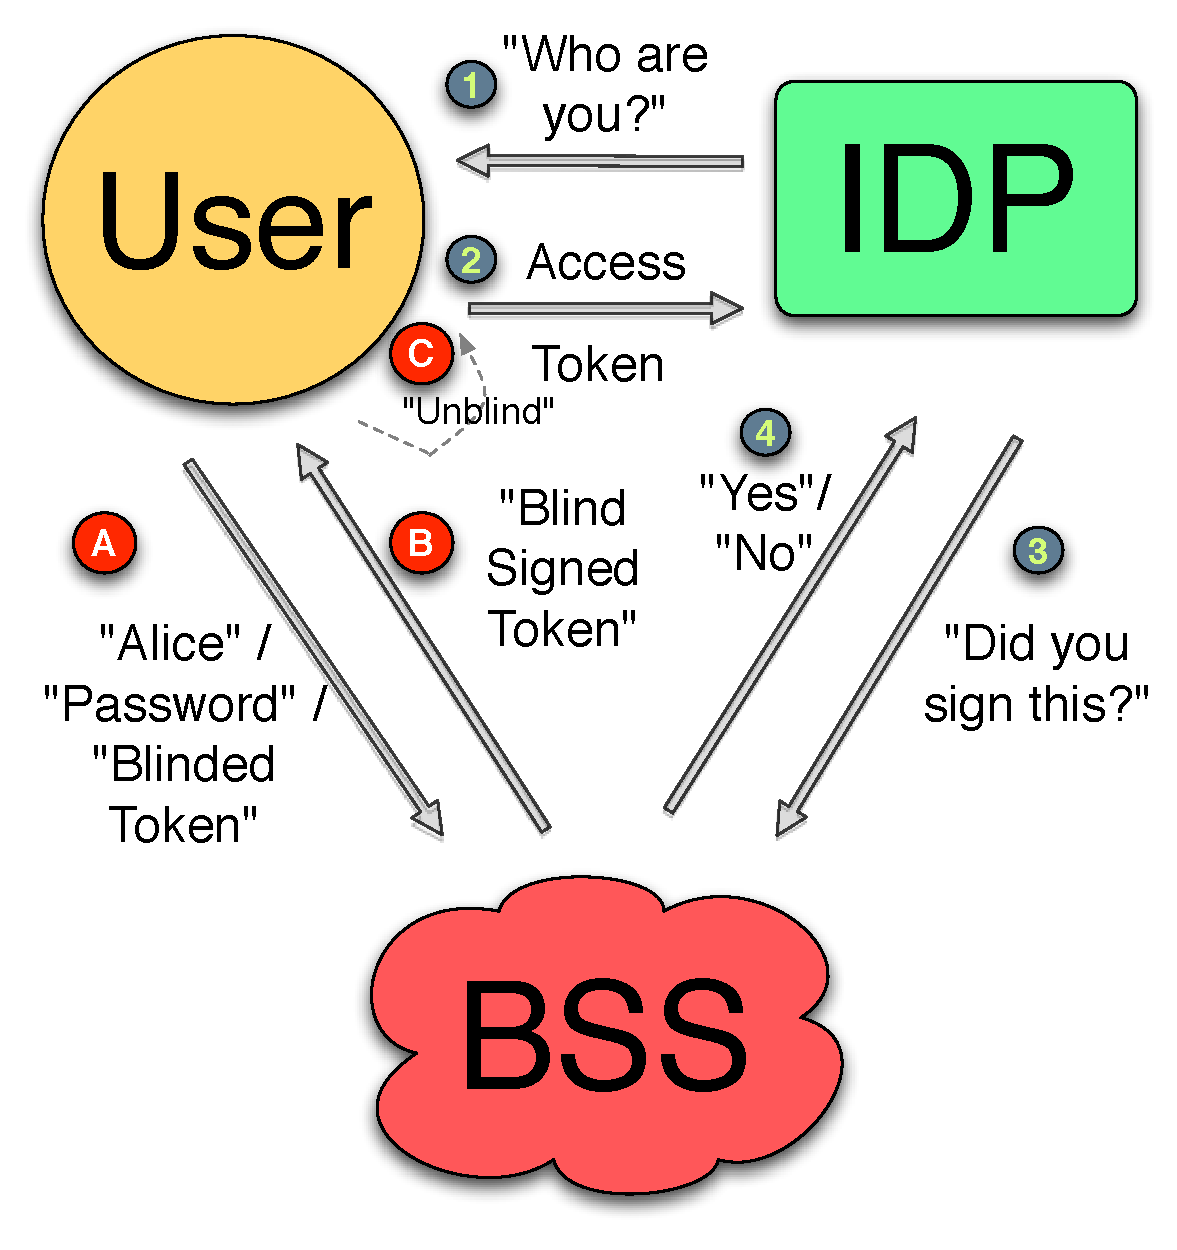
\includegraphics[scale=0.6]{figs/fig-bss-color.pdf}
  \caption{The user obtains an untraceable access token from the blind
    signature service prior to logging into a website. When his
    identity provider asks him to authenticate, he provides the access
    token instead of a username or password. The identity provider, in
    turn, verifies that the BSS signed the token. If the token has
    been validly signed, the provider authenticates the user to the
    website he is trying to visit.}
  \label{fig:bss}
\end{figure}
\end{comment}

\subsection{OpenID with PseudoID}

PseudoID is practical to implement in a web-based model appropriate
for OpenID. We have implemented a proof of concept blind signing
service and identity provider available at
\url{http://pseudoid.net}. The proof of concept blind signer is
implemented as a web service. Users visit the blind signer and 
prepare a blinded token signed with JavaScript (see Section
\ref{subsec:caveats} for a discussion of some security caveats). 

The blind signer will blindly sign this value and return it to the
user. This value is unblinded and stored as a cookie in the user's
browser. This cookie will be set on the identity provider's domain.

The identity provider itself may be slightly modified from existing
OpenID providers. It simply needs to read an access token from a
cookie on the user's browser, verify a signature on it, and return the
pseudonym it contains to a relying party. From the user's perspective,
this eliminates the need to retype a username and password on an
identity provider.

PseudoID identity providers are fully compatible with existing OpenID
relying parties. Existing relying parties do not have to change
anything about their current OpenID flow in order to be able to accept
users from private identity providers. From the perspective of the
relying party, a private identity provider is indistinguishable from a
regular provider. A private provider simply uses a different
authentication mechanism than most other identity providers, but it
still participates in the same federated login flow outlined in Figure
\ref{fig:fedlog}.

\subsection{Caveats of the proof of concept Implementation}
\label{subsec:caveats}

The proof of concept PseudoID implementation stores a user's access
tokens as cookies in the browser. This is not the ideal solution. Users 
who clear cookies frequently or use a private browsing mode would
lose their blinded access token. Cookies are also set in a
single browser, and thus it would be complicated to extend a user's
pseudonym across different machines.

There is also a security issue with setting a cookie on the identity
provider's domain. JavaScript executing on one domain cannot set a
cookie on another. The proof of concept PseudoID implementation must
make a call to the identity provider to set an unblinded cookie during
the setup phase. This means that access logs on the blind signer and
the identity provider could be joined to correlate the user's login
with the value that was set as a cookie. 

Even if logins are private, user requests can still be tied to a
particular IP address. Anonymization on the network level is an
independent risk and may be mitigated by the use of web proxies or
anonymous browsing technology like Tor \cite{Tor}. 

In practice, users are tracked more often by cookies than by IP 
addresses. One risk of the proof of concept system is that a malicious
blind signer or IDP may try to set tracking cookies on the user's
browser while they are logged in with their real identity. Thus, a
user would need to scrub all cookies except their access token from
their browser. This is not practical from a usability standpoint.

Another issue is that blinding and unblinding is being done with
JavaScript in the user's browser. This code must be trusted, otherwise
it could leak their identity. 

\section{Extensions and Future Work}

The caveats of the proof of concept PseudoID implementation make it
impractical for general use. There are both unresolved usability and
security issues which would need to be addressed in it and private
federated login systems in general.

\subsection{Simplified Cryptography in the Browser}

Modern browsers are equipped with support for a broad range of
cryptographic functionalities. Yet, it is difficult for a typical
web application to make use of it. In the case of PseudoID,
server-side JavaScript was used to blind and unblind tokens.

Using JavaScript is both inefficient and insecure. Basic cryptographic
functionality has to be reimplemented in JavaScript and interpreted,
rather than using the native cryptographic libraries already available
in the browser.

There is also a question of where the JavaScript code comes from. If
it is hosted on a server, it may later be substitued with malicious
code without the user's knowledge. For example, if the host of the
JavaScript code were compromised, an attacker could inject code to
leak the user's identity.

Browser crytpographic support could be made avaiable through
a browser plug-in or extension, but this is a barrier to adoption and
difficult to support on multiple platforms. PseudoID and many other
applications could benefit from a simple, standardized, and
cross-platform API to client-side cryptographic services.

\subsection{Browser Storage and Cross-Domain Communcation}

Another practical challenge in the proof of concept implementation was
communicating cryptographic tokens across domains subject to the
constraints of the \emph{same-origin policy}. In this case, a page on
the blind signer's domain cannot set a cookie on a different domain.

This was a difficulty because we wanted to set an \textit{unblinded}
token that was readable from the IDP's domain, but not visible to the
blind signer. The workaround was to load a hidden cross-domain
iframe. This technique was used to allow the blind signer to set a
cookie on the identity provider's domain. That represents a privacy
risk, since it would be easy to correlate logs between the blind
signer and the IDP.

PseudoID could benefit from a more flexible browser storage model than
cookies, and the means to pass messages from one domain to another
using the browser as an intermediary. Several features proposed in
HTML 5 may help facilitate this \cite{HTML5}.

\subsection{Selective Disclosure}

In the current version, PseudoID access tokens contain a user-selected
pseudonym and a random nonce. Tokens do not contain any meaningful
semantics nor any properties of the user's real identity. By using
zero-knowledge proofs, one may extend the blind signer to support
selective disclosure. There is a broad range of literature on this
topic \cite{Cha85,CaLy01,CaLy04,CHL05,CaGr08}.

The basic idea is that users will engage in a zero-knowledge proof
with the blind signer. They will prove that the contents of
blindly signed messages convey some meaningful data or have a proper
semantic form. For example, the user may prove that a blindly signed
message contains a bit value representing ``Is this user over 18 years
of age?'' that is true for their real identity, without revealing any
other information about the message.

Another example use is obtaining a token with an expiration time in
it. The user would prove to the blind signer that a blinded message
contains a valid expiration time, without revealing any other
knowledge of the message.

By allowing tokens to have these types of semantics, identity
providers will be able to offer more fine-grained access policies. In
the simple PseudoID system, IDPs can only verify a signature on a
token -- all they learn is that a blind signer signed it at some point
in time. If tokens had semantics, they could, for instance, only allow
access to users with tokens that were issued within some time period.

From a web-based implementation standpoint, performing zero-knowledge
proofs in the browser requires better support for both cryptography
and storing persistent values. While it is possible to implement
zero-knowledge proof systems with a JavaScript and cookie approach,
this would have the same security issues that the proof of concept
PseudoID implementation has.

\bibliography{pseudoid}
\bibliographystyle{acm}

\end{document}

% LocalWords:  login OpenID username
